\documentclass[12pt,a4paper]{article}
\usepackage{amsmath}
\usepackage[english]{babel}
\usepackage{graphicx}
\usepackage{listings}
\usepackage{fullpage}
\usepackage[T1]{fontenc}
\usepackage{enumerate}
\usepackage[makeroom]{cancel}
\usepackage{hyperref}
\usepackage{natbib}
\bibliographystyle{apj}

\lstdefinestyle{custompython}{
  belowcaptionskip=1\baselineskip,
  breaklines=true,
  frame=L,
  xleftmargin=\parindent,
  language=bash,
  basicstyle=\footnotesize\ttfamily,
  showstringspaces=false,
  %commentstyle=\itshape\color{purple!40!black},
  %keywordstyle=\itshape\color{green!40!black},
  %identifierstyle=\color{blue},
  %stringstyle=\color{orange},
}

\usepackage{todonotes}
\newcommand\TM[1]{\todo[color=green!40, inline, size=\small]{TM: #1}}
\newcommand\EW[1]{\todo[color=blue!40, inline, size=\small]{EW: #1}}
\newcommand\LC[1]{\todo[color=magenta!40, inline, size=\small]{LC: #1}}

\newcommand\Planck{{\it Planck}\ }
\newcommand\Cosmosis{{\it Cosmosis}\ }


% Roman numerals command
\makeatletter
\newcommand*{\rom}[1]{\expandafter\@slowromancap\romannumeral #1@}
\makeatother

% Some definitions for writing SN, SNe, SN Ia, and SNe Ia...
\newcommand{\sn}{\mbox{SN}}
\newcommand{\sne}{\mbox{SNe}}
\newcommand{\sna}{\mbox{SN \rom{1}a}}
\newcommand{\snea}{\mbox{SNe \rom{1}a}}

\author{
  Cheng, Lidens\\
  \texttt{lidenscheng@email.arizona.edu}
  \and
  McClintock, Tom\\
  \texttt{tmcclintock@email.arizona.edu}
  \and
  Wagoner, Erika\\
  \texttt{wagoner47@email.arizona.edu}
}
\title{Astr 513: Final Project}

\begin{document}
\maketitle

\section{Introduction}
\label{sec:Intro}
Type \rom{1}a supernovae (\snea{}) have been instrumental in the discovery 
of the accelerating expansion of the universe. Presently, {\sn} surveys continue 
to be pivotal in constraining cosmological parameters. In this paper, we present 
our analysis of comparing and combining {\sna} inference of cosmological parameters 
to those from other cosmological probes. In particular, we utilize the constraints 
from the Cosmic Microwave Background (CMB) and the Baryonic Acoustic Oscillations 
(BAO) that are gathered in \citet{planck2013}. We look at two cosmologies in our 
analysis: the $\Lambda \textnormal{CDM}$ universe and the wCDM universe. This 
paper is outlined as follows. In Section 2, the process and importance of {\snea} 
are summarized. A short description of the Planck mission is given in Section 3. 
Section 4 describe the two {\sna} surveys whose data we use for our analysis. The 
significance of using distance modulus data to constrain cosmological parameters 
is illustrated in Section 5. The CMB and BAO priors taken from \citet{planck2013} 
are also specified in Section 5. Our results and analysis on the benefit of omitting 
or including Bayesian priors from other cosmological probes 
are in Section 6 and Section 7.  

\section{Type \rom{1}a Supernovae}
\label{sec:SNIa}
A type \rom{1}a supernova is a supernova with very little hydrogen or
helium absorption. It is believed that the progenitor for these special
supernovae are white dwarfs that are part of a binary system. These white
dwarfs accrete mass from their companion stars or merge with a companion white
dwarf or neutron star, causing them to exceed the Chandrasekhar limit
($1.44 M_\odot$). When this happens, carbon and oxygen fusion begins in the
core, and the temperature increases. However, the white dwarf does not expand
and cool as a main sequence star would, since it is supported by degeneracy
pressure rather than thermal, so the core experiences a runaway fusion
reaction, releasing $\sim 10^{44}$ J of energy \citep[see, e.g.,][chap. 18.4]{ryden2010}, 
which is enough to overcome the gravitational energy and the star explodes. Because all 
\snea{} are caused by a similar reaction, they all have similar luminosities, and more 
importantly, the light curves all have the same shape: a sharp maximum followed by a smooth, 
gradual decay. Studying nearby \snea{} has shown that the rate of decline of the light curve 
is correlated to the peak luminosity, and this correlation has been calibrated using Cephied 
variable stars located in the same galaxies as nearby \sna{}. With this information, one can 
estimate peak luminosity of an \sna{} from its light curve, thereby providing a 
standard candle with which to measure distance. They were first used in this way in the 
1990s by two independent teams, the Supernova Cosmology Project and the Cal\'{a}n/Tololo 
Supernova Survey. It was using distances from \snea{} from these two projects that 
\citet{riess1998} and \citet{perlmutter1999} were able to discover the accelerating expansion 
rate of the Universe in 1998. 

\section{Planck 2015 Results}
\label{sec:planck}
In 2009 the European Space Agency launched the \Planck satellite in order
to measure the Cosmis Microwave Background with unparalleled precision.
By measuring the small anisotropies in the temperature of the CMB across
the entire sky one calculates the angular power spectrum, which can be
modeled using first principles (see, e.g., \citet{dodelson2003}).
By using a likelihood method similar to our own, the authors of
\citet{planck2013} estimated 14 nuisance parameters and 
six cosmological parameters, including the geometrical parameters,
$\Omega_M$, $\Omega_\Lambda$ and $\Omega_k$, that we use in our
{\sna} analysis. The only prior used by \citet{planck2013}
on cosmological parameters was from the WMAP result \citep{wmap2011}
for the optical depth $\tau$. We do not use this parameter
in our {\sna} model.

\citet{planck2013} report marginalized
posterior distributions for all parameters,
which we report in Table~XXX. This prior is implemented
in the planck2015 module implemented in \Cosmosis \citep{cosmosis}.

\section{Data}
\label{sec:data}
Our {\sna} data is compiled from the samples analyzed in 
\citet{betoule2014} and \citet{rest2014}. In the following subsections, 
we will specify the surveys and detail the composition of the two samples. 
Additionally, we will describe the publicly released data from the two papers.

\subsection{The JLA sample}
\label{sec:betoule}
\citet{betoule2014} define their ``joint light-curve analysis'' (JLA) 
sample, a total of 740 \snea{} compiled from a combination of 
data from the Sloan Digital Sky 
Survey (SDSS), the Supernova Legacy Survey (SNLS), the Hubble Space 
Telescope (HST), and several other experiments. The 613 SDSS \snea{} 
come from the SDSS supernova survey (SDSS-SNS) of SDSS-II \citep{sako2014} 
with redshifts of $0.05 < z < 0.4$, and 374 of them are selected from those 
that were confirmed in the spectroscopic follow-up. The rest of the 
\sne{} come from the compilation by \citet{conley2011}, which includes 
242 spectroscopically confirmed \snea{} from SNLS at redshifts $0.2 < z < 1$, 
14 \snea{} from HST at very high redshifts of $0.7 < z < 1.4$, and 123 
low redshift ($z < 0.08$) from a variety of sources. We made use of the 
publicly available distance moduli, redshifts, and covariance 
matrix provided by \citet{betoule2014}\footnote{Data is available 
for download via 
\url{http://cdsarc.u-strasbg.fr/viz-bin/qcat?J/A+A/568/A22}}. 
We note that the distance moduli are binned, so that they are only computed and 
given on a grid of redshifts. The distance modulus can then be well 
approximated by a piecewise linear function of $\log(z)$ that is given 
in a single redshift bin $z_b \le z < z_{b+1}$ as 
\citep[see][Appendix E.1]{betoule2014}
%
\begin{equation}
\label{eq:binnedMu}
\bar{\mu}(z) = (1 - \alpha) \mu_b + \alpha \mu_{b+1},
\end{equation}
%
where they have defined 
$\alpha = \log\left(\frac{z}{z_b}\right)/\log\left(\frac{z_{b+1}}{z_b}\right)$ 
and $\mu_i$ is the distance modulus at control point $z_i$. 
Therefore, the data and covariance matrix are merely given at the 
31 control points log-spaced in the redshift range $0.01 < z < 1.3$.

\subsection{The Pan-STARRS1 sample}
\label{sec:rest}
\citet{rest2014} uses the first 1.5 year of the first telescope of 
the Panoramic Survey Telescope and Rapid Response System (Pan-STARRS1) 
and a compilation of low-redshift {\sna} studies. The low-redshift 
sample consists of {\snea} collected by Calan/Tololo (Hamuy et al. 1996a), 
CfA1 (Riess et al. 1999), CfA2 (Jha et al. 2006), CfA3 (Hicken et al. 2009a), 
CSP (Contreras et al. 2010), and CfA4 (Hicken et al. 2012). After 
three quality cuts, 113 spectroscopically confirmed {\snea} from 
Pan-STARRS1 ($0.03 < z < 0.65$) and 222 light curves from 197 
low-redshift {\snea} are used for cosmological analysis. 

The publicly available data from \citet{rest2014} contains all light 
curves, light curve fit information, covariance matrix, and each {\sn} 
host information.\footnote{Data can be accessed at 
\url{http://ipp0012.ifa.hawaii.edu/SN1aLC/}}. For our analysis, we 
utilized the redshifts, distance moduli, and covariance matrix of the 
final sample of 310 {\snea} or 335 light curves.

\subsection{Covariances}
\label{sec:covariances}
The publicly released covariance matrix from \citet{rest2014} 
is comprised of systematic and statistical errors for the final sample. 
The total covariance matrix is defined as 
$\mathbf{C}= \mathbf{D}_{\textnormal{stats}}+\mathbf{C}_{\textnormal{sys}}$. The 
statistical matrix has only diagonal elements, which take into account errors 
in light curve fit parameters and intrinsic scatter due to luminosity and 
color variation. These statistical errors are added in quadratures. The 
systematics, defined in \citet{scolnic2014}, include flux calibration errors, 
selection effects, light curve fitting, host galaxy relations, Milky Way 
extinction corrections, and coherent velocity flows. Calculating the systematic 
matrix involves varying a systematic parameter and determining the difference 
between the original distance and the new distance. The systematic covariance 
between {\sn} $i$ and {\sn} $j$ is 
%
\begin{equation}
  \label{eq:RestCovMatrix}
  C_{ij,\textnormal{sys}}=\displaystyle \sum_{k = 1}^K \left(\frac{\partial \mu_i}{\partial S_k}\right)\left(\frac{\partial \mu_j}{\partial S_k}\right)\left(\sigma_{S_k}\right)^2,
\end{equation}
%
where the summation is over $K$ systematics, $\sigma_{S_k}$ is each 
systematic error magnitude, and $\partial \mu$ is the difference in 
distance modulus from varying a systematic parameter.

\citet{betoule2014} choose to first calculate the covariance 
matrix $\mathbf{C}_{\mathbf{\eta}}$ of the 3 light curve fit-parameters $\mathbf{\eta}$ 
by adding the individual covariance matrices they get from statistical errors propagated 
from light-curve fit uncertainties and 7 sources of systematic uncertainties 
they consider from their photometric calibartion, light-curve model uncertainty, 
bias correction, a mass step uncertainty introduced when correcting magnitudes due 
to host mass, Galactic extinction, peculiar velocities, and contamination by 
non-\sna{}. They then propagate these errors to the distance modulus and use three 
terms to account for uncertainty in cosmological redshift by the equation
%
\begin{equation}
\label{eq:BetouleCovMatrix}
\mathbf{C} = \mathbf{A} \mathbf{C}_\mathbf{\eta} \mathbf{A}^\dag + \mathrm{diag}\left(\frac{5 \sigma_z}{z \log 10}\right)^2 + \mathrm{diag}\left(\sigma_{\mathrm{lens}}^2\right) + \mathrm{diag}\left(\sigma_{\mathrm{coh}}^2\right),
\end{equation}
%
where $\mathbf{A}$ is the matrix of coefficients in the distance modulus, 
and redshift uncertainty is accounted for in the first diagonal term due to 
peculiar velocities, the second due to magnitude variation from gravitational lensing, 
and the third from intrinsic \sn{} magnitude variation not included in other terms. 
They use $c \sigma_z = 150 \mathrm{km}\, \mathrm{s}^{-1}$, 
$\sigma_{\mathrm{lens}} = 0.055 \times z$, and a value of $\sigma_{\mathrm{coh}}$ for each 
survey found using a restricted log-likelihood technique. The elements of the covariance 
matrix available online are calculated on the redshift control points $z_b$ as 
described in \S \ref{sec:betoule}.

For both of these data sets, the covariance matrix can be visualized using a related
quantity known as the correlation matrix $Corr$. When two quantities are (anti)correlated,
the value of one quantity (decreases)increases when the other quantity increases.
If the variables one has measured are independent, then the correlation between
different variables should be $\approx0$.

A correlation matrix for $N$ variables is $N\times N$ in size, and the $ij$th
element is the correlation between the $i$th and $j$th variables. Therefore, 
the correlation matrix for \citet{betoule2014} is $31\times31$, while
for \citet{rest2014} is $335\times335$.

The correlation matrix is calculated from the covariance matrix according to
%
\begin{equation}
  \label{eq:correlation}
  Corr_{i,j} = \frac{\mathbf{C}_{i,j}}{\sqrt{\mathbf{C}_{i,i}}\sqrt{\mathbf{C}_{j,j}}}.
\end{equation}
%
Note that the correlation of a variable with itself is 1 by definition.
The correlation matrices for both of our data sets can be seen below in
figures \autoref{fig:cmatrix_betoule} and \autoref{fig:cmatrix_rest}.
%
\begin{figure}
  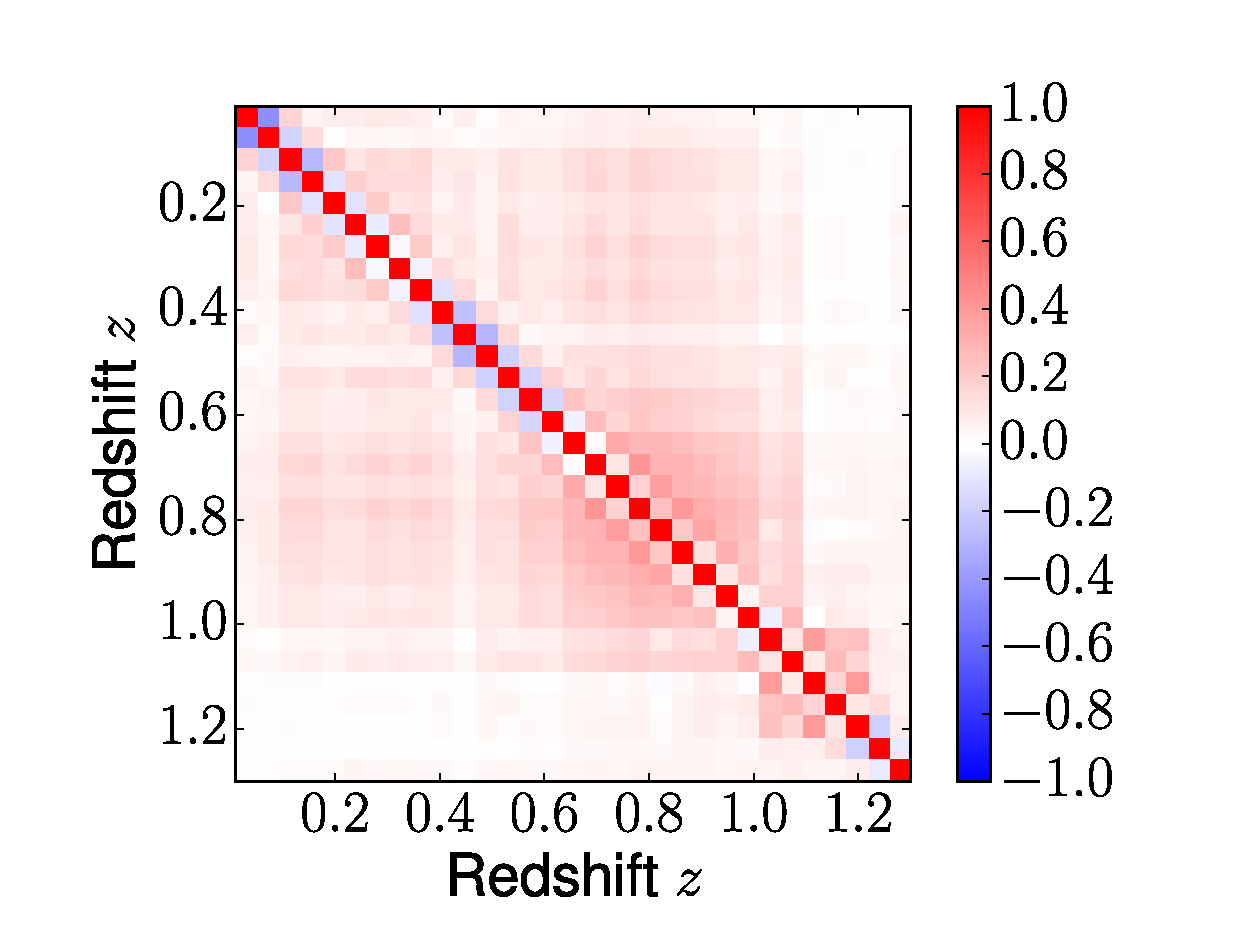
\includegraphics[width=0.8\linewidth]{figures/Betoule_correlation.eps}
  \caption{Correlation matrix of $\mu_0(z)$ from the
    \citet{betoule2014} sample. Overall very few correlations exist between
    samples, likely due to the averaging over redshift bins.}
  \label{fig:cmatrix_betoule}
\end{figure}
%
\begin{figure}
  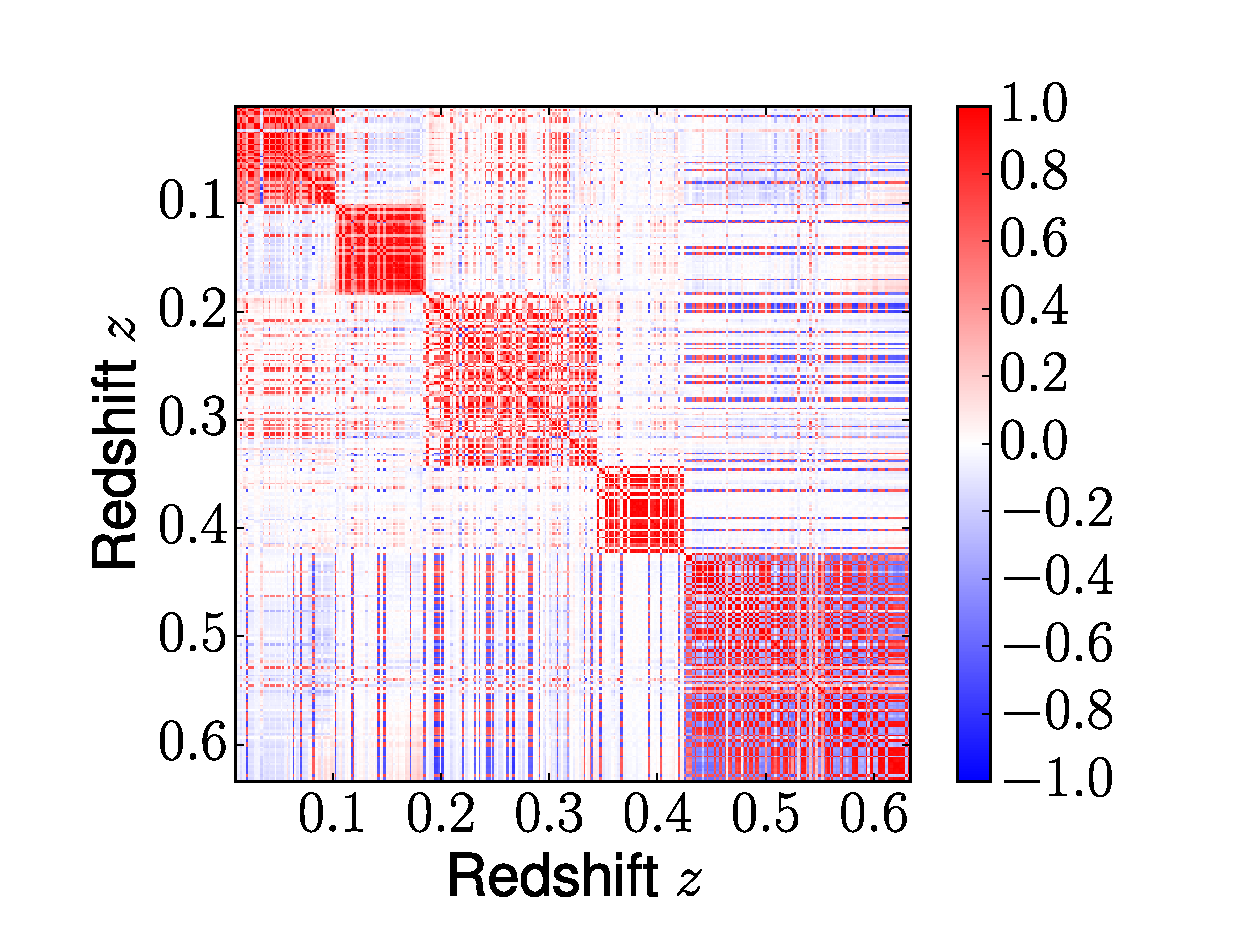
\includegraphics[width=0.8\linewidth]{figures/Rest_correlation.eps}
  \caption{Correlation matrix of $\mu_0(z)$ from the
    \citet{rest2014} sample. Significant correlation exist between
    different samples due to dependencies on systematic variables
    as seen in \autoref{eq:RestCovMatrix}.}
  \label{fig:cmatrix_rest}
\end{figure}

\section{Distance Modulus Model}
\label{sec:model}
The main objective of \citet{betoule2014} and \citet{rest2014} is 
to place constraints on cosmological parameters $\Omega_M$, $\Omega_\Lambda$, 
$\Omega_k$, and $w$. In order to so, we must examine the relationship between distance 
modulus and cosmology. The distance modulus $\mu$ is determined from 
the luminosity distance $d_L$ by 
%
\begin{equation}
  \label{eq:mu_dL}
  \mu=5 \log\left(\frac{d_L}{1 \mathrm{Mpc}}\right)+25. 
\end{equation}
%
The luminosity distance depends on the cosmology by 
%
\begin{equation}
\label{eq:luminosityDistance}
d_L(z; w, \Omega_M, \Omega_\Lambda, H_0)= (1+z)|\Omega_k|^{-1/2}\mathcal{S}_{k}\displaystyle\left[c|\Omega_k|^{1/2}\int_{0}^{z}\frac{dz'}{H(z')}\right],
\end{equation}
%
where $\Omega_k \equiv 1-\Omega_M-\Omega_{\Lambda}$. The function 
$\mathcal{S}_{k}$ depends on the curvature density $\Omega_k$ in that 
\[
    \mathcal{S}_{k}= 
\begin{cases}
    \text{sin}(x),&  \Omega_k < 0\\
    x,& \Omega_k = 0\\
    \text{sinh}(x),& \Omega_k > 0
\end{cases}.
\]
The function $H(z)$ is expressed as 
%
\begin{equation}
  \label{eq:hubbleFunction}
  H(z)= H_0\displaystyle\left[\Omega_M(1+z)^3+\Omega_{\Lambda}(1+z)^{3(1+w)}+\Omega_k(1+z)^2\right]^{1/2},
\end{equation}
%
where the Hubble constant $H_0$ can be written in terms of a 
dimensionless Hubble parameter $h$ by $H_0=100h \mathrm{km\ s^{-1}Mpc^{-1}}$.

Two cosmologies are of interest to us: the $\Lambda \textnormal{CDM}$ 
universe and the wCDM universe. In the $\Lambda \textnormal{CDM}$ 
universe, $w=-1$ and constraints are placed on $\Omega_M$ and $h$. 
The wCDM universe is a one-parameter extension of $\Lambda \textnormal{CDM}$ 
in which $w$ is an arbitrary parameter for a constant dark energy 
equation of state. In wCDM, constraints are placed on $\Omega_M$, $w$, 
and $h$. In both cosmologies, the universe is spatially flat 
($\Omega_k = 0$) and thus $\Omega_{\Lambda}=1-\Omega_M$. 

\subsection{Likelihood}
\label{sec:likelihood}
Using the above model for the distance modulus allows us to write a
probability that a model can generate our data:
%
\begin{eqnarray}
  \label{eq:likelihood}
  P(\mu(z)|\mathrm{cosmo}) = \frac{1}{\sqrt{2\pi|\mathbf{C}|}}\exp
  \left[-\frac{1}{2} \sum_{i,j=0}^{N_{samples}}\left(\mu(z) - \mu_{\mathrm{model}}(z)\right)_i 
    \mathbf{C}^{-1}_{i,j}\left(\mu(z) - \mu_{\mathrm{model}}(z)\right)_j\right]
\end{eqnarray}
%
where $\mathbf{C}$ is the full covariance matrix between all of the $N_{samples}$ 
in the data, and $\mathrm{cosmo}$ represents the cosmology that we are investigating
(e.g. flat $\Lambda$CDM, $wCDM$, etc.). 
This is not the full picture though, since we must employ
Bayes' Theorum in order to include any priors on our choice of 
parameters and recover the posterior distribution function of our
parameters given our data
%
\begin{equation}
  \label{eq:posterior}
  P(\mathrm{cosmo}|\mu(z)) = P_{prior}(\mathrm{cosmo}) P(\mu(z)|\mathrm{cosmo}).
\end{equation}
%
For this work we investigate a combination of priors. \Cosmosis is implemented
in a way that requires the user to provide bounds on the parameter space, which we
detail for each parameter in \autoref{tab:priors}
Within those bounds, we investigated using a flat prior $P_{prior}=1$ and
\Planck priors.

\begin{table}
  \centering
  \caption{Bounds on cosmological parameters 
    entering \autoref{eq:posterior}. Our sampler requires
    bounds in order to both populate the parameter space with
    parallelized samplers and to calculate an appropriate width
    for the step size.}
  \label{tab:priors}
  \begin{tabular}{lll}
    Parameter & Description & Bounds \\ \hline
    $h$ & Hubble constant$/100$ & $[0,2]$ \\
    $\Omega_M$ & Matter fraction at $z=0$ & $[0,1]$ \\
    $w$ & Dark energy E.O.S. & $[-2,0]$\\
  \end{tabular}
\end{table}

\subsection{Planck Priors}
\label{sec:planck_priors}
\TM{The only thing we really require is a corner plot of {\it just} the priors.}

\section{Results}
\label{sec:results}
\TM{Discuss the results and show the corner plots. Example plot included.
  We should have one corner plot without priors and one with priors.}
\LC{Not sure where to put why we couldn't do the full analysis of Rest's data. 
  I'm putting it here for now.}
A complete analysis using the data from \citet{rest2014} is not done 
in our paper since there are several issues with the publicly released 
data. It is not apparent which uncertainties belonged to the statistical 
covariance matrix since only the systematic covariance matrix is clearly 
presented. Moreover, intrinsic dispersion of the data and photometric errors 
of the distances depend on nuisance parameters in addition to the covariances 
between the fit parameters. Fine-tuning nuisance parameters places a significant 
time restraint on our work and is beyond the scope of this paper. For these reasons, 
we only present the results for \citet{rest2014} that do not include the priors 
from \citet{planck2013}. 

\begin{figure}
  \centering
  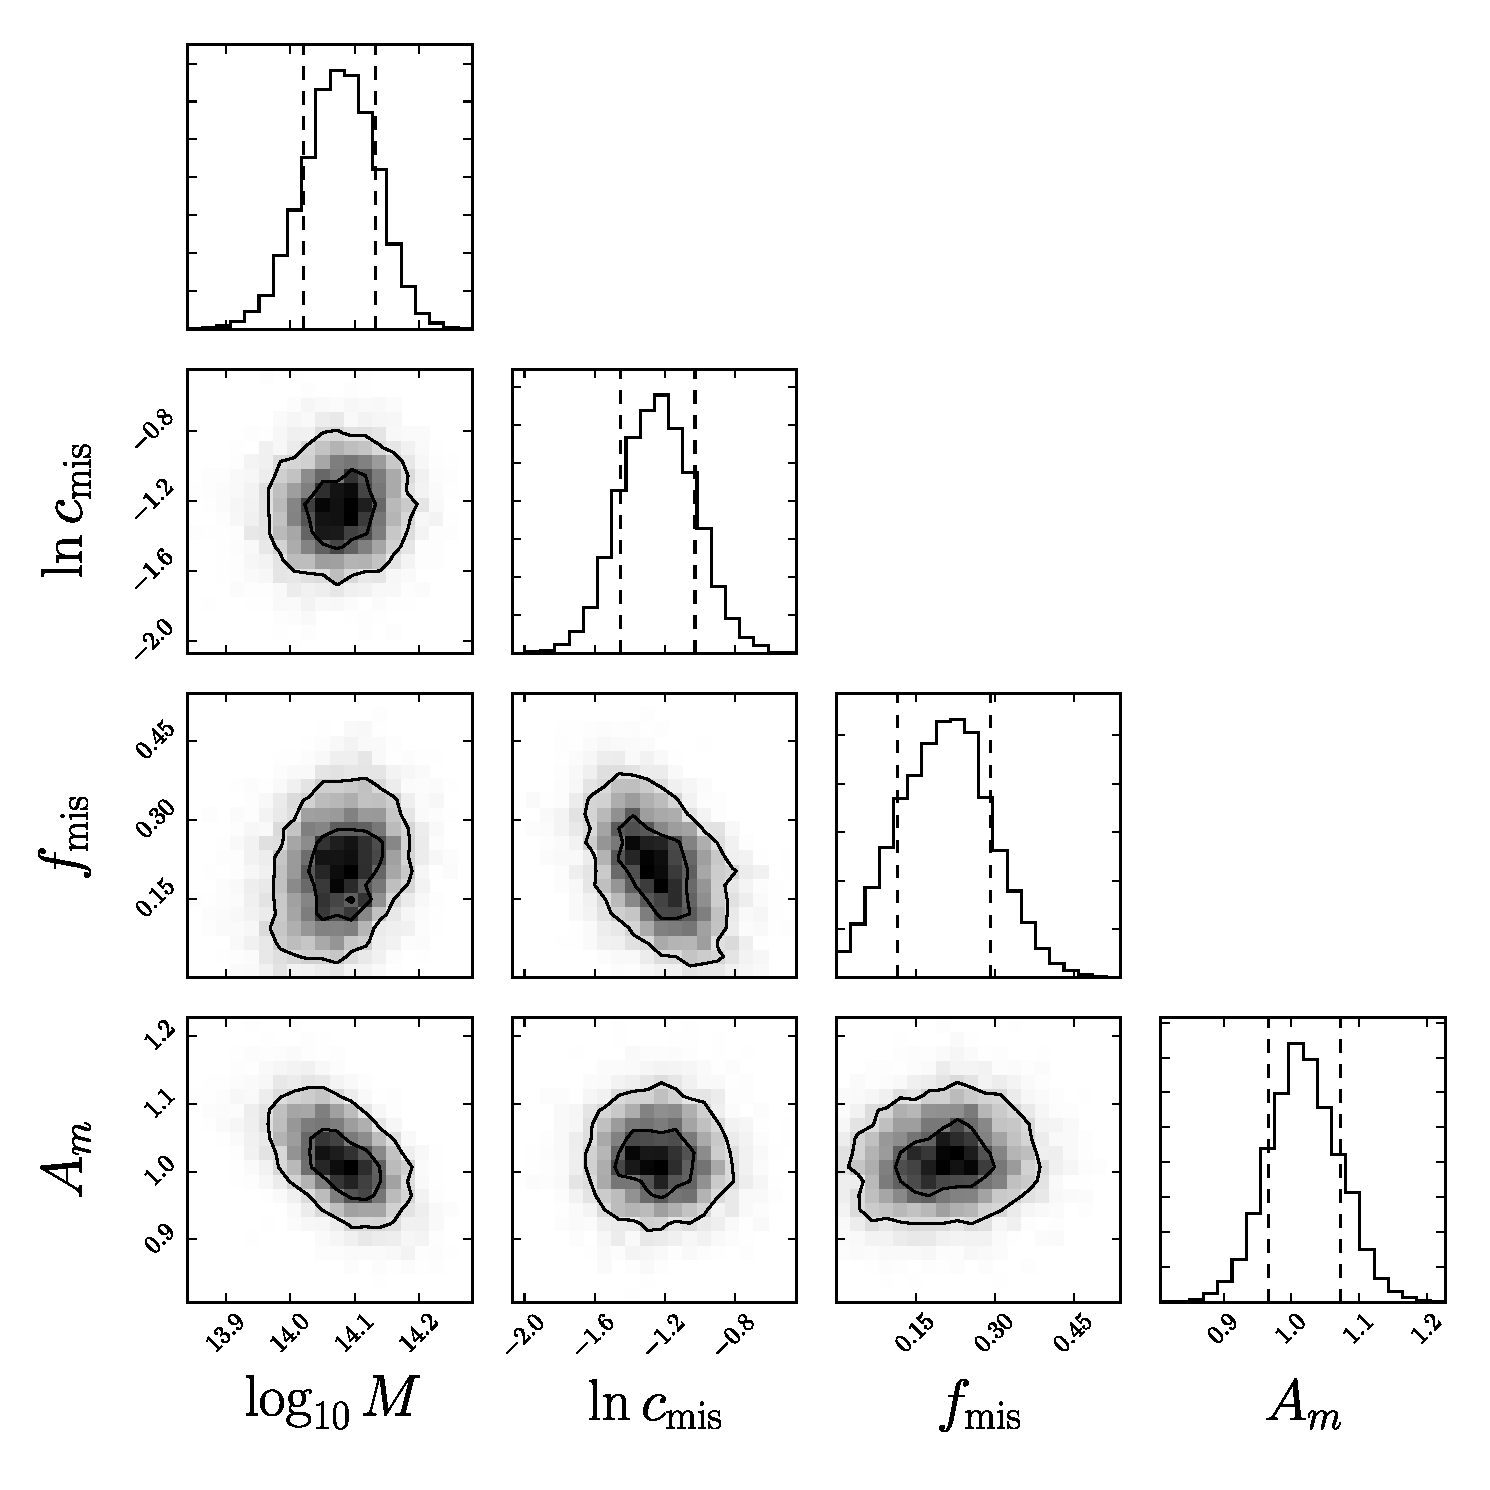
\includegraphics[width=0.5\linewidth]{figures/corner_example.eps}
  \caption{Example corner plot.}
  \label{fig:corner}
\end{figure}

\section{Conclusions}
\label{sec:conclusions}
\TM{Talk about how the inclusions if priors changes the analysis.
  State whether the priors are strong or uninformative.}

\bibliography{msbib}

\end{document}
